\chapter{Resultados}
\label{cap:resultados}

% Responde a ¿qué se encontró?, ¿qué se desarrolló?, ¿qué resultados se obtuvieron?

\section{Validación del pipeline}
\label{sec:res-validacion}

Antes de interpretar las agendas de los partidos conviene establecer en qué
medida las estimaciones de texto del pipeline son confiables. Los análisis de
los capítulos siguientes descansan por completo sobre las predicciones temáticas
de la clasificación supervisada (sección~\ref{sec:metodo-manifestoberta}): si esa
capa no reprodujera de forma razonable una codificación experta, cualquier
hallazgo sobre énfasis o soporte sería un artefacto del clasificador antes que
una propiedad de los datos. Por eso esta primera sección de resultados reporta la
evidencia de validez del método antes de presentar los análisis sustantivos.

La validación aprovecha que los manifiestos son el \emph{único} corpus del
proyecto con una codificación humana de referencia ---el código MARPOR asignado
manualmente a cada cuasi-frase (\texttt{cmp\_code})--- y se organiza en los
niveles complementarios diseñados en la sección~\ref{sec:metodo-validacion}. El
primero es una validación \emph{interna} a nivel de documento: contrasta la
categoría predicha contra la categoría humana sobre el mismo material. Los demás
operan a nivel de partido, una vez que las categorías se proyectan sobre el eje
izquierda--derecha mediante el índice RILE: primero comprobando que la
agregación del modelo reproduce la de los códigos humanos, y luego confrontando
ambas con un \emph{benchmark} independiente de expertos, el \emph{Chapel Hill
Expert Survey} (CHES) 2019 \cite{jolly2022ches, ches2019data}.

\subsection{Validación del clasificador contra MARPOR humano}
\label{sec:res-val-clasificador}

La primera comprobación enfrenta las predicciones de ManifestoBERTa
\cite{manifestoberta2024} sobre los manifiestos de 2017 contra el
\texttt{cmp\_code} humano, cuasi-frase a cuasi-frase. El contraste se realiza
sobre las \textbf{3.430} cuasi-frases con código humano utilizable (del total de
3.801 del corpus, descartando las que no tienen un código MARPOR numérico
asignable). Sobre esa base (Cuadro~\ref{tab:val-clasificador}), la clasificación
automática alcanza una
\textbf{exactitud de la categoría principal (top-1) del $58{,}3\,\%$}, que sube
al \textbf{$82{,}0\,\%$ al considerar las tres categorías más probables
(top-3)}. Como la asignación de dominio se obtiene del primer dígito del código,
la \textbf{exactitud a nivel de dominio} ---más robusta por agrupar categorías
afines--- es del \textbf{$70{,}3\,\%$}. El desempeño promediado por categoría,
medido con el \textbf{\emph{macro} F1, es de $0{,}44$}, valor que refleja la
fuerte asimetría del esquema: las categorías frecuentes se clasifican bien,
mientras que varias categorías raras arrastran el promedio.

\begin{table}[H]
\centering
\caption{Validación del clasificador ManifestoBERTa contra el código humano
MARPOR (\texttt{cmp\_code}) sobre los manifiestos de 2017
($n = 3.430$ cuasi-frases con código utilizable). La última columna reproduce el
desempeño reportado por los autores del modelo (\emph{model card}) como
referencia.}
\label{tab:val-clasificador}
\begin{tabular}{@{}l r r@{}}
\toprule
\textbf{Métrica} & \textbf{Valor obtenido} & \textbf{\emph{Model card}} \\
\midrule
Exactitud top-1 (categoría exacta) & $58{,}3\,\%$ & $57{,}0\,\%$ \\
Exactitud top-3 (categoría en las 3 principales) & $82{,}0\,\%$ & $81{,}0\,\%$ \\
Exactitud a nivel de dominio (1--7) & $70{,}3\,\%$ & --- \\
\emph{Macro} F1 (56 categorías) & $0{,}44$ & --- \\
\bottomrule
\end{tabular}
\end{table}

Estas cifras son \textbf{consistentes con la \emph{model card}} del modelo
(top-1 $57{,}0\,\%$, top-3 $81{,}0\,\%$), lo que indica que la transferencia
directa al francés político de la XV legislatura no degrada el desempeño
respecto del reportado por sus autores. La brecha entre el acierto top-1 y el
top-3, y entre el de categoría y el de dominio, es coherente con dos rasgos ya
anticipados en la metodología: el esquema MARPOR asume una sola etiqueta por
documento ---lo que penaliza a las cuasi-frases multitemáticas--- y las
confusiones se concentran entre categorías de dominios contiguos (por ejemplo,
entre economía y bienestar, o entre bienestar y grupos sociales), de modo que el
error se atenúa al leer los resultados a nivel de dominio.

\subsection{Validación posicional: RILE frente a CHES}
\label{sec:res-val-ches}

La validación interna confirma que el modelo reproduce la codificación humana
sobre el mismo material, pero no garantiza que las estimaciones \emph{agregadas}
midan algo externamente reconocible. Para examinarlo, las categorías MARPOR se
proyectan sobre el eje izquierda--derecha mediante el índice \textbf{RILE} de
Laver y Budge \cite{laver1992party}, calculado por partido según se describe en
la sección~\ref{sec:metodo-validacion}. El RILE se computa de dos maneras sobre
las mismas cuasi-frases ---a partir de los códigos predichos por el modelo y a
partir de los códigos humanos--- y se contrasta con la ubicación
izquierda--derecha (\texttt{lrgen}) que el CHES~2019 asigna a cada partido. Dado
que el número de partidos emparejables es pequeño, se reporta siempre el $n$ y se
privilegia la correlación de rangos de Spearman ($\rho$).

\begin{table}[H]
\centering
\caption{Correlación entre el RILE estimado y la ubicación izquierda--derecha del
CHES~2019 (\texttt{lrgen}), en las tres capas de validación y en los
diagnósticos. Se reportan el coeficiente de rangos de Spearman ($\rho$), el de
Pearson ($r$) y el número de partidos ($n$).}
\label{tab:val-ches}
\begin{tabular}{@{}l r r r@{}}
\toprule
\textbf{Comparación} & \textbf{Spearman $\rho$} & \textbf{Pearson $r$} & \textbf{$n$} \\
\midrule
A) Modelo frente a humano & $0{,}79$ & $0{,}85$ & $10$ \\
B) Modelo frente a CHES (externa) & $0{,}38$ & $0{,}42$ & $8$ \\
Techo) Humano frente a CHES & $0{,}76$ & $0{,}75$ & $8$ \\
\midrule
\multicolumn{4}{@{}l}{\emph{Diagnósticos sobre la capa B}} \\
\quad Modelo frente a CHES, partidos con $\geq 100$ cuasi-frases & $0{,}89$ & $0{,}72$ & $6$ \\
\quad Modelo frente a CHES, excluyendo RN & $0{,}36$ & $0{,}37$ & $7$ \\
\quad Modelo frente a CHES, eje económico (\texttt{lrecon}) & $0{,}57$ & $0{,}43$ & $8$ \\
\bottomrule
\end{tabular}
\end{table}

El diseño descompone la validez en \textbf{tres capas}
(Cuadro~\ref{tab:val-ches}), que separan el error del
modelo del error del método. La primera, \emph{modelo frente a humano}, compara
el RILE estimado por el modelo con el derivado de los códigos humanos sobre las
mismas cuasi-frases: mide cuánto se aparta el clasificador automático de la
codificación experta una vez agregado por partido. Pese a una exactitud
por-cuasi-frase de apenas el $58{,}3\,\%$, esta capa alcanza una correlación
\textbf{$\rho \approx 0{,}79$} ($n=10$): los errores de clasificación, en gran
medida, se \emph{cancelan} al promediar por partido, de modo que la posición
agregada se preserva. La segunda capa, \emph{modelo frente a CHES}, es la
validación externa propiamente dicha y arroja una correlación más modesta,
\textbf{$\rho \approx 0{,}38$} ($n=8$). La tercera, \emph{humano frente a CHES},
fija el
\textbf{techo} alcanzable por el método ---cuánto coinciden dos
patrones de referencia independientes, la codificación humana de MARPOR y la
encuesta de expertos--- y se sitúa en \textbf{$\rho \approx 0{,}76$} ($n=8$). Que
el techo no sea cercano a uno es esperable, porque ambos instrumentos miden cosas
relacionadas pero no idénticas: el RILE resume \emph{énfasis temático} y el CHES,
\emph{posición percibida}.

La distancia entre la segunda capa ($\rho \approx 0{,}38$) y el techo ($\rho
\approx 0{,}76$) no se debe a un fallo sistemático del modelo, sino a unos pocos
partidos con muy poco texto codificado. Al restringir la comparación a los
partidos con \textbf{al menos 100 cuasi-frases} ---umbral de fiabilidad habitual
en MARPOR--- la correlación externa sube a \textbf{$\rho \approx 0{,}89$}
($n=6$), un valor que se sitúa dentro del rango de la propia codificación humana
de MARPOR. Conviene precisar que este $\rho$ y el techo no se calculan sobre la
misma muestra ---el techo se estima sobre los ocho partidos emparejables y este
diagnóstico sobre los seis con suficiente texto---, por lo que no son
directamente comparables; lo que indican, en conjunto, es que cuando hay
suficiente texto por partido la posición estimada desde el discurso se aproxima a
la de los expertos. El caso que más arrastra la correlación en la muestra
completa es el del PCF, cuyo manifiesto aporta solo 39 cuasi-frases y produce una
estimación de RILE inestable. La Figura~\ref{fig:rile-ches} ilustra esta capa
externa sobre los ocho partidos emparejables: se aprecia una tendencia
ascendente, aunque modesta ($\rho \approx 0{,}38$) y muy condicionada por el
desajuste del PCF.

\begin{figure}[H]
\centering
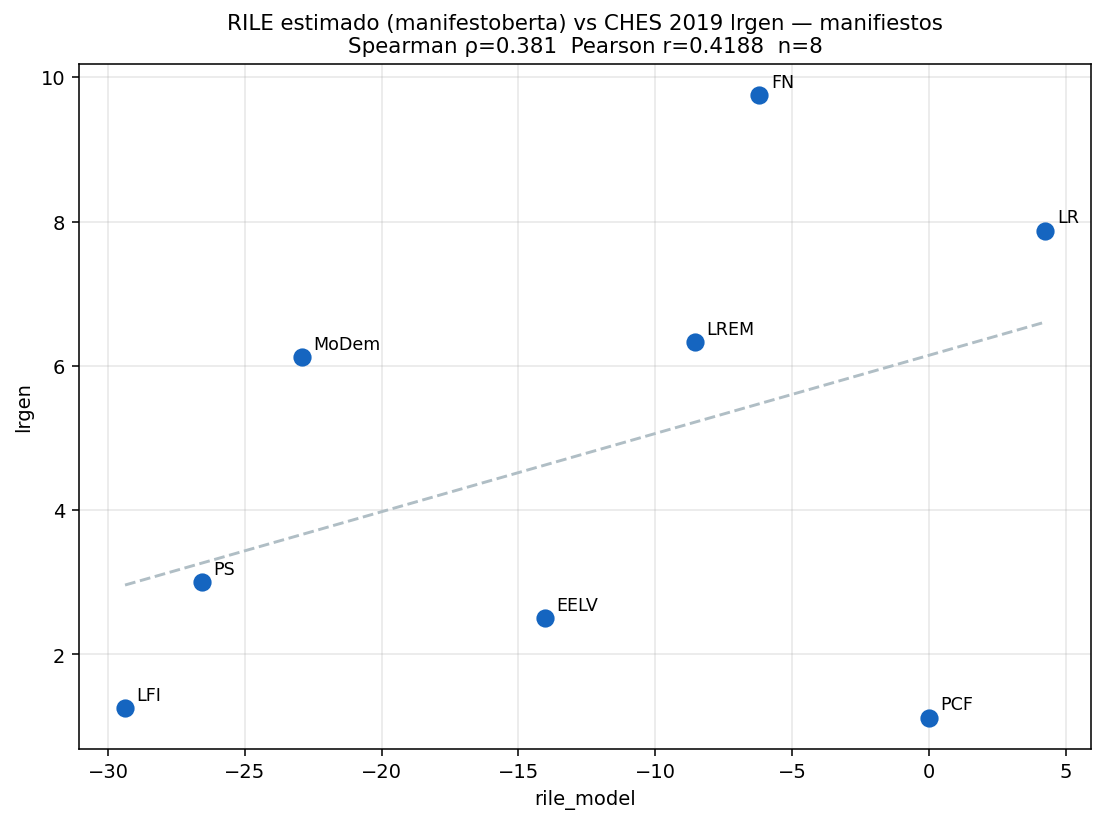
\includegraphics[width=0.82\linewidth]{imagenes/scatter_rile_vs_ches.png}
\caption{RILE estimado por el modelo (eje horizontal) frente a la ubicación
izquierda--derecha del CHES~2019 (\texttt{lrgen}, eje vertical) para los ocho
partidos emparejables (capa B, $\rho \approx 0{,}38$, $n=8$). La línea
discontinua marca la tendencia.}
\label{fig:rile-ches}
\end{figure}

\subsection{Alcance de la validación}
\label{sec:res-val-alcance}

La evidencia anterior debe leerse con varias salvedades que acotan su alcance.
La más importante es que \textbf{la validación solo puede hacerse sobre los
manifiestos}, porque son el único canal con codificación humana MARPOR y el
único con un \emph{benchmark} de expertos comparable. No existe un \emph{ground
truth} equivalente para tuits, intervenciones, leyes o enmiendas, de modo que la
calidad de la clasificación en esas arenas se asume por transferencia desde el
desempeño observado en los manifiestos, no se mide directamente.

En segundo lugar, todas estas correlaciones descansan sobre \textbf{un
número muy pequeño de partidos} (entre 6 y 10, y solo entre 6 y 8 en las capas
que involucran al CHES), por lo que son sensibles a casos individuales y deben
interpretarse como indicios de validez y no como estimaciones precisas; de ahí el
uso de correlación de rangos y el reporte sistemático del $n$. A esa fragilidad contribuyen además las \textbf{muestras
pequeñas} de algunos manifiestos: el PCF aporta apenas 39 cuasi-frases y el PS,
79, por lo que sus posiciones estimadas son solo indicativas. Se suma un
\textbf{desfase temporal} asumido: la referencia de expertos corresponde a 2019
y los manifiestos a las elecciones de 2017, una diferencia de dos años que puede
introducir discrepancias menores sin invalidar la comparación.

Por último, conviene reiterar que el RILE se emplea aquí \textbf{únicamente como
instrumento de validación externa}, no como eje del análisis. Es un índice
posicional unidimensional, frágil y ciego a la dirección del enunciado, por lo
que resulta inadecuado para caracterizar agendas ricas y multidimensionales. El
análisis sustantivo de los partidos, que se desarrolla en las secciones
siguientes, se construye en cambio sobre el \emph{énfasis temático} ---las
distribuciones completas de categorías y dominios MARPOR \cite{marpor_mp_v5}---
y no sobre este eje izquierda--derecha. En síntesis, la validación respalda usar
las predicciones del pipeline como base de los análisis temáticos: el
clasificador reproduce la codificación humana al agregar por partido y, con
suficiente texto, recupera posiciones que se aproximan a las de un panel
independiente de expertos.

\section{Las bases de datos construidas}
\label{sec:res-bases}
% Cobertura y volumen por corpus; tablas resumen.

\section{Agenda declarada: el canal define de qué se habla}
\label{sec:res-declarada}
% Hallazgo transversal: manifiestos = programa (Welfare); tweets/hemiciclo =
% meta-política (Political System). La firma distintiva de cada partido persiste.

\subsection{Manifiestos}
\label{sec:res-manifestos}
% Firmas por partido (EELV->ambiente, PS->bienestar, FN->nación, ...). Caveats de muestra.
% \begin{figure}[H] \centering \includegraphics[width=\linewidth]{...} \caption{...} \end{figure}

\subsection{Twitter}
\label{sec:res-tweets}
% Political System estalla; LFI como megáfono anti-gobierno; NI -> ley y orden.

\subsection{Hemiciclo}
\label{sec:res-hemiciclo}
% La oposición fiscaliza (305 Autoridad Política); LREM defiende gestión (303).

\section{Agenda revelada por el voto}
\label{sec:res-revelada}

\subsection{Dos capas del voto: posicional y temática}
\label{sec:res-dos-capas}
% Leyes invierten la estructura de apoyo respecto de enmiendas (gobierno vs oposición).

\subsection{Cohesión: quién vota en bloque}
\label{sec:res-cohesion}
% LFI la más disciplinada; NI y LT las menos cohesionadas (bolsas mixtas).

\subsection{Clivajes ideológicos en las enmiendas}
\label{sec:res-clivajes}
% Eje cultural (Fabric of Society) vs. libertades (Freedom & Democracy); consenso exterior.

\section{Declarado vs. revelado: ¿votan lo que dicen?}
\label{sec:res-declarado-revelado}
% Tipología por celda (énfasis respaldado / coherencia negativa / oposicional);
% coherencia agregada débil; la estructura interpretable está en los signos por celda.
